% 
% Annual Cognitive Science Conference
% Sample LaTeX Paper -- Proceedings Format
% 

% Original : Ashwin Ram (ashwin@cc.gatech.edu)       04/01/1994
% Modified : Johanna Moore (jmoore@cs.pitt.edu)      03/17/1995
% Modified : David Noelle (noelle@ucsd.edu)          03/15/1996
% Modified : Pat Langley (langley@cs.stanford.edu)   01/26/1997
% Latex2e corrections by Ramin Charles Nakisa        01/28/1997 
% Modified : Tina Eliassi-Rad (eliassi@cs.wisc.edu)  01/31/1998
% Modified : Trisha Yannuzzi (trisha@ircs.upenn.edu) 12/28/1999 (in process)
% Modified : Mary Ellen Foster (M.E.Foster@ed.ac.uk) 12/11/2000
% Modified : Ken Forbus                              01/23/2004
% Modified : Eli M. Silk (esilk@pitt.edu)            05/24/2005
% Modified : Niels Taatgen (taatgen@cmu.edu)         10/24/2006
% Modified : David Noelle (dnoelle@ucmerced.edu)     11/19/2014

%% Change "letterpaper" in the following line to "a4paper" if you must.

\documentclass[10pt,letterpaper]{article}

\usepackage{cogsci}
\usepackage{pslatex}

% create hyperlinks
\usepackage{hyperref} 
\hypersetup{colorlinks=true,citecolor=blue} % no ugly boxes

\usepackage{apacite}

% additional packages
\usepackage{graphicx}
\usepackage{subcaption}
\usepackage{nicefrac}
\usepackage{xspace}
\usepackage{tikz}
\usetikzlibrary{shapes.geometric}
\usepackage{pgfplots}
\usepackage{stmaryrd}



%  set the font 
\usepackage{amsmath,amssymb}

\newcommand{\rar}{\rightarrow}
\newcommand{\biar}{\leftrightarrow}
\DeclareMathOperator*{\argmax}{arg\,max}
\newcommand{\ud}{\,\mathrm{d}}
\newcommand{\intp}[1]{\llbracket #1 \rrbracket}
\newcommand{\rsa}{\acro{rsa}}
\newcommand{\intpw}[1]{\llbracket \mbox{#1} \rrbracket}
\newcommand{\pair}[1]{\langle #1 \rangle}
\newcommand{\soc}{\ensuremath{\theta}\xspace}



\title{What do eye movements in the visual world reflect? A case study from adjectives}
 
\author{{\large \bf Ciyang Qing, Daniel Lassiter$^*$, Judith Degen$^*$} \\ 
  {$\{$qciyang, danlassiter, jdegen$\}$@stanford.edu} \\
  Department of Linguistics, Stanford University\\
  460 Serra Mall, Stanford, CA 94305, USA}


\begin{document}

\maketitle


\begin{abstract}
%The abstract should be one paragraph, indented 1/8~inch on both sides,
%in 9~point font with single spacing. The heading ``{\bf Abstract}''
%should be 10~point, bold, centered, with one line of space below
%it. This one-paragraph abstract section is required only for standard
%six page proceedings papers. Following the abstract should be a blank
%line, followed by the header ``{\bf Keywords:}'' and a list of
%descriptive keywords separated by semicolons, all in 9~point font, as
%shown below.

A common dependent measure used in visual-world eye-tracking experiments is the proportion of looks to a visually depicted object in a certain time window after the onset of the critical stimulus. When interpreting such data, a common assumption is that looks to the object reflect the listener's belief that the object is the intended target referent. While this is intuitively plausible (at least for paradigms in which the task requires selecting a referent), relatively little is known about how exactly the proportion of looks to an object is related to a listener's current belief about that object. Here, we test a simple, explicit linking hypothesis: the proportion of looks to an object correlates with the probability that the listener assigns to the object being the target. To test this hypothesis, we supplement the eye-tracking data from \citeA{LeffelXiangKennedy2016:Imprecision-is-Pragmatic-} with an offline incremental decision task to measure participants' beliefs about the intended referent at various points in the unfolding sentence, and assess the extent to which these beliefs predict the eye-tracking data.
The results suggest that the degree to which an object is believed to be the referent is only one factor that affects eye movements in referential tasks. 
Preliminary free production data we have collected for the scenes suggests that utterance expectations also play a role. 
We discuss methodological implications of these results for experimental linguistics.

\textbf{Keywords:} 
eye-tracking; visual world; linking functions; gradable adjectives; vagueness; imprecision; semantics; pragmatics
\end{abstract}



%The entire contribution of a proceedings paper (including figures,
%references, and anything else) can be no longer than six pages.
%
%The text of the paper should be formatted in two columns with an
%overall width of 7 inches (17.8 cm) and length of 9.25 inches (23.5
%cm), with 0.25 inches between the columns. Leave two line spaces
%between the last author listed and the text of the paper. The left
%margin should be 0.75 inches and the top margin should be 1 inch.
%\textbf{The right and bottom margins will depend on whether you use
%  U.S. letter or A4 paper, so you must be sure to measure the width of
%  the printed text.} Use 10~point Times Roman with 12~point vertical
%spacing, unless otherwise specified.
%
%The title should be in 14~point, bold, and centered. The title should
%be formatted with initial caps (the first letter of content words
%capitalized and the rest lower case). Each author's name should appear
%on a separate line, 11~point bold, and centered, with the author's
%email address in parentheses. Under each author's name list the
%author's affiliation and postal address in ordinary 10~point type.
%
%Indent the first line of each paragraph by 1/8~inch (except for the
%first paragraph of a new section). Do not add extra vertical space
%between paragraphs.


\section{Introduction}

Eye-tracking experiments using the \emph{visual world paradigm} \cite<VWP,>{tanenhaus1995} are widely used in linguistics \cite{SedivyEtAl1999:Achieving-Incremental-Semantic-, LeffelXiangKennedy2016:Imprecision-is-Pragmatic-}. In standard VWP tasks, participants view displays of four objects while listening to spoken sentences while their eye movements are monitored (see Fig.~\ref{fig:sedivyetal}). A commonly used dependent measure for evaluating whether experimental conditions -- that reflect theoretically interesting conditions -- differ from each other is the difference in \emph{proportion of looks to a visually depicted object in a certain time window after the onset of a critical stimulus} across condition. When interpreting such data, a common assumption is that looks to the object reflect the listener's belief that the object is the intended target referent. While this is intuitively plausible (at least for paradigms in which the task requires selecting a referent, cf. \citeNP{SalverdaTanenhaus2017:The-Visual-World-Paradigm}), relatively little is known about how exactly the proportion of looks to an object is related to a listener's current belief about that object (but see \citeNP{AllopennaEtAl1998:Tracking-the-Time-}). Understanding the relation between looks and beliefs is crucial for the theoretical interpretation of eye movement data for the purpose of linguistic theory-building. Here, we test a simple, explicit linking hypothesis: \textbf{the proportion of looks to an object correlates with the probability that the listener assigns to the object being the target}. 
To test this hypothesis, we supplement the eye-tracking data from \citeA{LeffelXiangKennedy2016:Imprecision-is-Pragmatic-} with an offline \emph{incremental decision task} to measure participants' beliefs about the intended referent at various points in the unfolding sentence, and assess the extent to which these beliefs predict the eye-tracking data.
The results suggest that the degree to which an object is believed to be the referent is only one factor that affects eye movements in referential tasks. 
Preliminary free production data we have collected for the scenes suggests that utterance expectations also play a role. 
We discuss methodological implications of these results for experimental linguistics.


\begin{figure}[h]
  \centering
  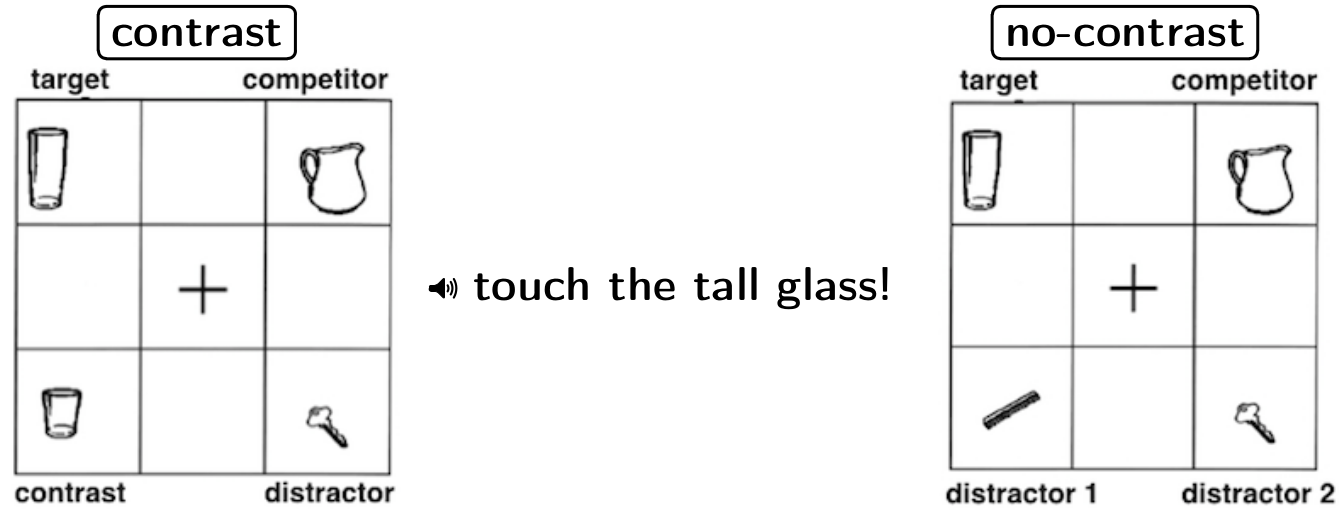
\includegraphics[width=.5\textwidth]{plots/SedivyEtAl1999.png}
  \caption{Visual world paradigm used in Sedivy et al., 1999}
  \label{fig:sedivyetal}
\end{figure}

\vspace{-2ex}

\section{A case study: gradable adjectives}

\begin{figure*}[ht]
  \centering
  \begin{subfigure}[b]{0.2\textwidth}
    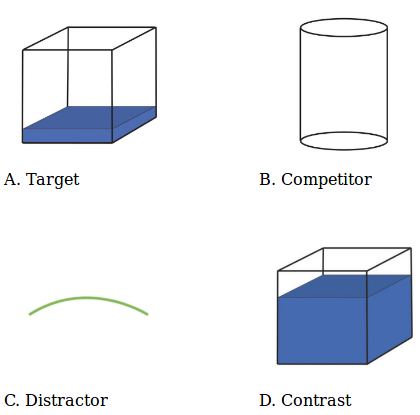
\includegraphics[width=\textwidth]{plots/scene15c.png}
    \caption{Max (\emph{empty}), contrast}
    \label{fig:maxcontrast}
  \end{subfigure}
  \qquad
  ~ %add desired spacing between images, e. g. ~, \quad, \qquad, \hfill etc. 
  %(or a blank line to force the subfigure onto a new line)
  \begin{subfigure}[b]{0.2\textwidth}
    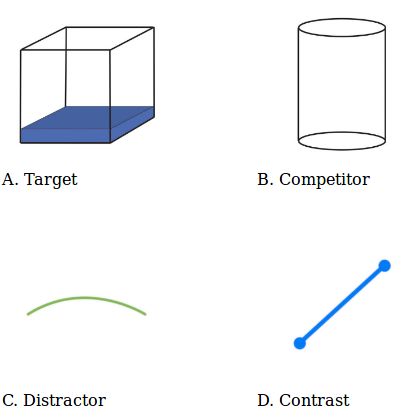
\includegraphics[width=\textwidth]{plots/scene15nc.png}
    \caption{Max (\emph{empty}), no contrast}
    \label{fig:maxnocontrast}
  \end{subfigure}
  \qquad
  \begin{subfigure}[b]{0.2\textwidth}
    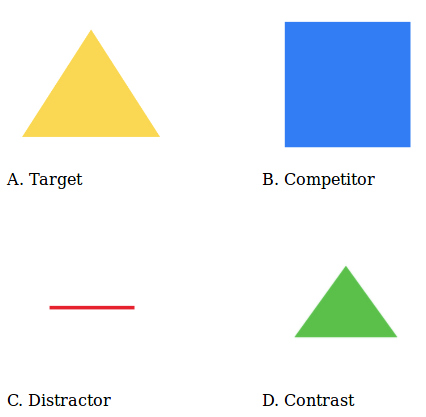
\includegraphics[width=\textwidth]{plots/scene33c.png}
    \caption{Rel (\emph{big}), contrast}
    \label{fig:relcontrast}
  \end{subfigure}
  \qquad
  ~ %add desired spacing between images, e. g. ~, \quad, \qquad, \hfill etc. 
  %(or a blank line to force the subfigure onto a new line)
  \begin{subfigure}[b]{0.2\textwidth}
    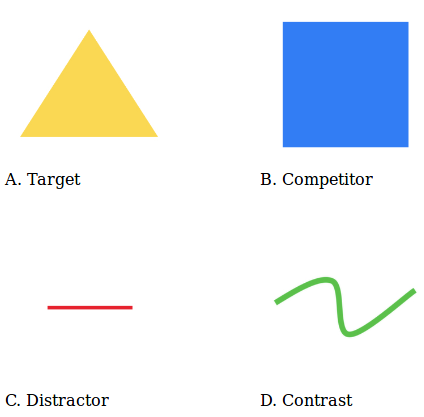
\includegraphics[width=\textwidth]{plots/scene33nc.png}
    \caption{Rel (\emph{big}), no contrast}
    \label{fig:relnocontrast}
  \end{subfigure}
  %  ~ %add desired spacing between images, e. g. ~, \quad, \qquad, \hfill etc. 
  %  %(or a blank line to force the subfigure onto a new line)
  %  \begin{subfigure}[b]{0.2\textwidth}
  %    \includegraphics[width=\textwidth]{mouse}
  %    \caption{A mouse}
  %    \label{fig:mouse}
  %  \end{subfigure}
  \caption{Stimuli used in Leffel et al., 2016. Critical sentences are of the form ``click on the [adj] [noun]''}
  \vspace{-2ex}
  \label{fig:stimuli}
\end{figure*}

\begin{figure}[ht]
  \centering
  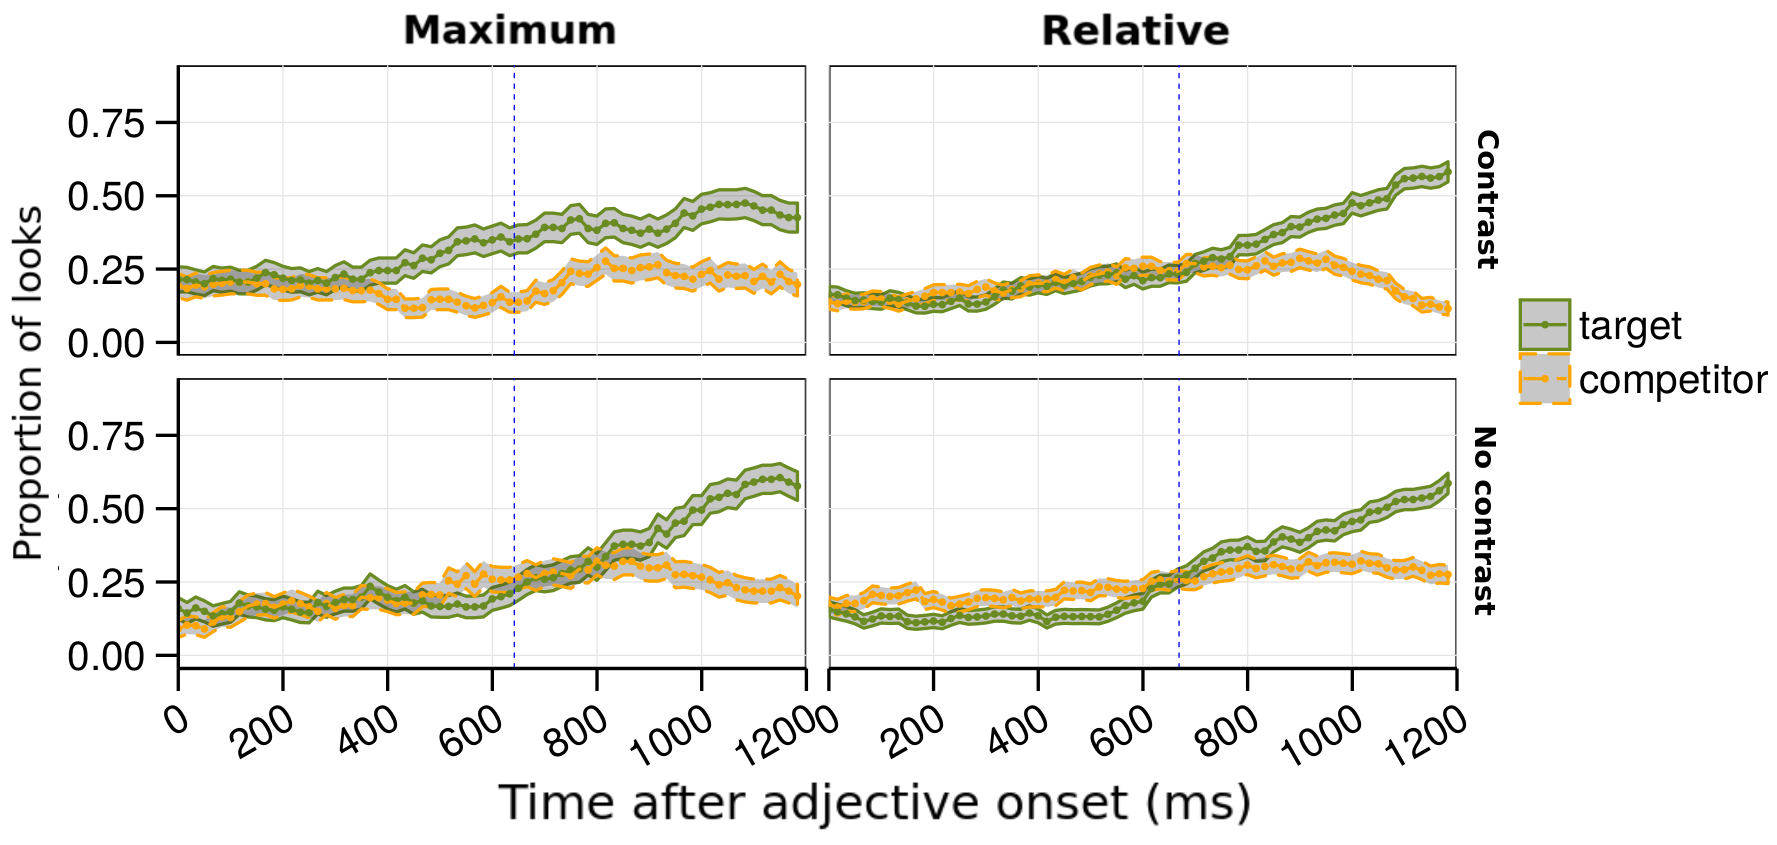
\includegraphics[width=.5\textwidth]{plots/leffeletalresults.png}
  \caption{Proportions of looks on targets and competitors for different adjective types (columns)
    across contrast conditions (rows) from Leffel et al.'s (2016) visual world study. Blue lines indicate 200ms after average noun onset.}
  \vspace{-4ex}
  \label{fig:leffelEtAlResults}
\end{figure}



We tested the above linking hypothesis on an eye movement dataset that was collected with the intention of informing the debate over semantic theories of gradable adjectives such as \emph{empty} and \emph{big}. We  recap the theoretical motivation for the experiment before focusing on testing the linking hypothesis.

According to degree-based approaches to the meaning of gradable adjectives \cite<e.g.,>{Kennedy2007:Vagueness-and-Grammar}, 
 an object $o$ satisfies a gradable adjective $A$ iff $o$'s degree of $A$-ness exceeds
 a standard of comparison $\theta$. There are empirical differences between how \emph{big} and \emph{empty} are interpreted. 
\emph{Relative} adjectives such as \emph{big} and \emph{tall} are \emph{context-sensitive} and \emph{vague}.
In contrast, \emph{maximum} adjectives such as \emph{empty} and \emph{straight} are not (or much less) \emph{vague}: strictly
 speaking, a glass is empty iff it exhibits a maximum amount of emptiness (i.e., it is completely empty).\footnote{There is a third class of gradable adjectives such as \emph{bent} and \emph{dirty}, which only
  requires a minimum degree as the standard $\theta$. 
Following \citeA{LeffelXiangKennedy2016:Imprecision-is-Pragmatic-}, we do not consider such adjectives.
}

The maximum/relative distinction is complicated by the fact that speakers often use these adjectives in an \emph{imprecise} way. For example, it is often acceptable to call a glass empty when in fact there is still a little water in it.

There is a consensus in the literature that the interpretation of relative adjectives involves 
 resolution of the standard $\theta$ based on contextual information.
However, theories differ in terms of how they analyze maximum adjectives and in particular their imprecise uses. 
According to recent probabilistic approaches, imprecise uses of maximum adjectives can be captured by a unified 
 model of the contextual resolution of $\theta$, and the differences between maximum and relative adjectives
 follow from different world knowledge about the various properties denoted by gradable adjectives
 \cite{LassiterGoodman2013:Context-Scale-S,LassiterGoodman2015:Adjectival-vagu,QingFranke2014:Gradable-Adject,QingFranke2014:Meaning-and-Use}.
Following \citeA{LeffelXiangKennedy2016:Imprecision-is-Pragmatic-}, we call such approaches the 
 \emph{semantic hypothesis about imprecision} (\textbf{HS}).
In contrast, \citeA{LeffelXiangKennedy2016:Imprecision-is-Pragmatic-} proposes a \emph{pragmatic hypothesis}
 (\textbf{HP}), according to which maximum adjectives always use maximum degrees as $\theta$ and 
 imprecise uses are due to an additional pragmatic mechanism that relaxes their strict literal meanings. 
 
\citeA{LeffelXiangKennedy2016:Imprecision-is-Pragmatic-} attempted to use VWP to adjudicate between these two hypotheses. 
They conducted a variant of \citeauthor{SedivyEtAl1999:Achieving-Incremental-Semantic-}'s
 \citeyear{SedivyEtAl1999:Achieving-Incremental-Semantic-} experiment  (Fig.~\ref{fig:sedivyetal}),  in which participants saw displays of four objects and 
 their task was to take actions according to auditory stimuli 
 such as ``touch the tall glass.''
Among the four objects, there was one that uniquely satisfied the full DP \emph{the tall glass}
(the \emph{target} object). 
In addition, there was a \emph{competitor} object that satisfied the adjective but not the noun 
 (the tall pitcher).
In half of the displays (the \emph{contrast} condition) there was an object (the \emph{contrast}) that satisfied the noun but not the adjective (e.g., the short glass). 
The rest of the objects were \emph{distractors} that satisfied neither the adjective nor the noun (e.g., the
 comb and the key). The main finding, now a classic effect, is what has since been termed the \emph{Referential Contrast Effect} \cite{Sedivy2003:Pragmatic-Versus-Form-}:  there was a difference in proportions of looks between the contrast and no-contrast conditions when only the adjective information was available, such that listeners looked more to the target in the presence of a contrast member, presumably as a result of pragmatic reasoning about the adjective only being necessary to distinguish two members of a contrast pair.
 
Building on \citeA{SedivyEtAl1999:Achieving-Incremental-Semantic-}, \citeA{LeffelXiangKennedy2016:Imprecision-is-Pragmatic-}'s study leveraged the Referential Contrast Effect to test the processing of both maximum
 and relative gradable adjectives (Fig.~\ref{fig:stimuli}).
Crucially, the competitor object always exhibited a higher degree of the property denoted by the adjective 
 than the target, and in the case of maximum adjectives the competitor satisfied the adjective perfectly
 (e.g., the perfectly empty cylinder in Fig.~\ref{fig:stimuli}). 
Thus, in the case of maximum adjectives the target object was described by the adjective only in 
 an imprecise way.


% Exp 1 setting and click data

%\begin{figure*}[ht]
%  \centering
%  \begin{subfigure}[b]{0.25\textwidth}
%    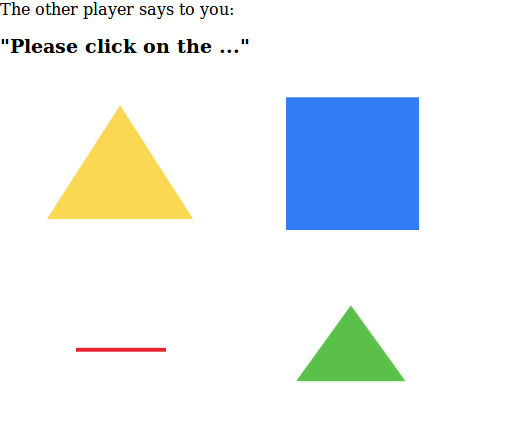
\includegraphics[width=\textwidth]{plots/MTurkExpPrior.png}
%    \caption{Prior}
%    \label{fig:mturkprior}
%  \end{subfigure}
%  ~ %add desired spacing between images, e. g. ~, \quad, \qquad, \hfill etc. 
%  %(or a blank line to force the subfigure onto a new line)
%  \begin{subfigure}[b]{0.25\textwidth}
%    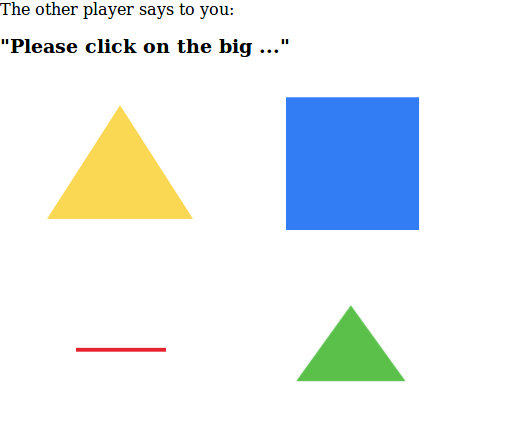
\includegraphics[width=\textwidth]{plots/MTurkExpAdj.png}
%    \caption{Adjective}
%    \label{fig:mturkadj}
%  \end{subfigure}
%  \begin{subfigure}[b]{0.25\textwidth}
%    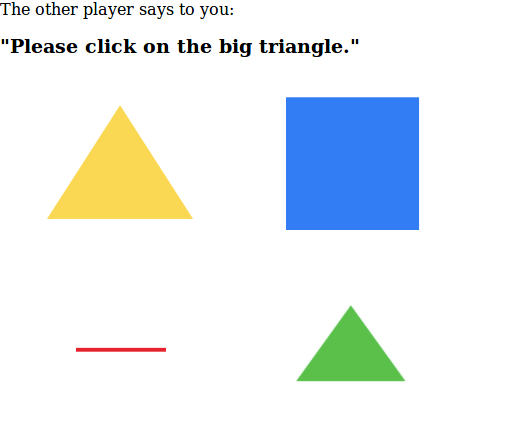
\includegraphics[width=\textwidth]{plots/MTurkExpNoun.png}
%    \caption{Noun}
%    \label{fig:mturknoun}
%  \end{subfigure}
%  %  ~ %add desired spacing between images, e. g. ~, \quad, \qquad, \hfill etc. 
%  %  %(or a blank line to force the subfigure onto a new line)
%  %  \begin{subfigure}[b]{0.2\textwidth}
%  %    \includegraphics[width=\textwidth]{mouse}
%  %    \caption{A mouse}
%  %    \label{fig:mouse}
%  %  \end{subfigure}
%  \caption{The 3 windows in the incremental decision task}
%  \label{fig:mturk}
%\end{figure*}

\begin{figure}[ht]
  \centering
    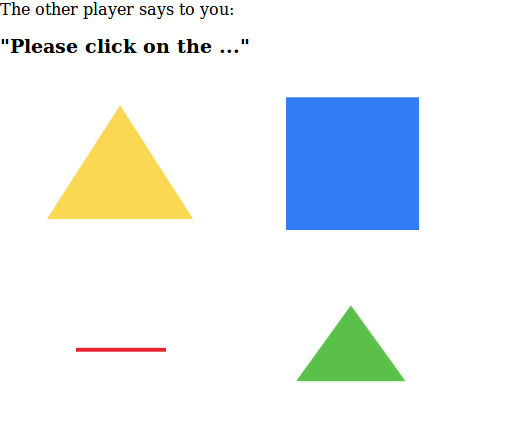
\includegraphics[width=.35\textwidth]{plots/MTurkExpPrior.png}
    \vspace{-4ex}
  \caption{Visual stimulus in the prior window in the incremental decision task. In the adjective window, the adjective (e.g., \emph{big}) was additionally displayed; in the noun window, the noun (e.g., \emph{triangle}) was also displayed.}
      \vspace{-2ex}
  \label{fig:mturk}
\end{figure}

They observed a Referential Contrast Effect  for maximum adjectives but not for relative adjectives (Fig.~\ref{fig:leffelEtAlResults}).
They concluded that this favors \textbf{HP}, based on the following reasoning.
(i) If \textbf{HS} were true, the resolution strategy of $\theta$ 
should be the same for both maximum and relative adjectives and hence the same processing pattern is expected for both types of adjectives.
(ii) If \textbf{HP} were true, the resolution strategies of $\theta$ should be different for maximum
 and relative adjectives and hence their processing patterns should differ as well.
(iii) Given that RCE was observed only for maximum adjectives, the empirical finding is compatible with \textbf{HP} but not \textbf{HS}.

This kind of reasoning is commonplace in experimental semantics/pragmatics and we would like to probe some of the premises involved. In this paper, we focus on (i). For probabilistic approaches, the resolution strategy of $\theta$ is specified at the 
 computational level \cite{marr1982}.
Given that having the same computational mechanism does not generally guarantee the same processing pattern 
 (e.g., it takes longer to calculate the sum of two 30-digit numbers than 3-digit numbers, even though the
 underlying computational mechanisms can well be the same), (i) is not valid without additional assumptions.
In fact, two types of additional assumptions are needed: (a) an assumption about the computational product of the resolution strategy, e.g., the contrast manipulation will affect probabilistic beliefs about the intended referent in the same way for both types of adjectives, and (b) a linking hypothesis: an assumption about the link between the computational product (probabilistic belief about the referent) and the processing pattern (proportion of looks), e.g., the proportion of looks to an object reflects the probability that the listener 
assigns to the object being the intended referent (in the same way for both types of adjectives). 

 
Given the central role that listeners' beliefs about the intended referent play in the above assumptions, 
we directly measured these beliefs using a novel offline paradigm (which we refer to as the  \emph{incremental decision task}).
We will focus on the linking hypothesis in (b) for two main reasons.
First, existing probabilistic theories mentioned above are designed for \emph{descriptive} uses of 
 gradable adjectives (e.g., ``John is tall'') and do not directly make predictions about the 
 \emph{referential} uses in \citeauthor{LeffelXiangKennedy2016:Imprecision-is-Pragmatic-}'s experiment,
Therefore it is unclear whether the assumption in (a) holds.
But even if it does, the linking hypothesis in (b) still needs to hold for (i) to be the case.
More importantly, the linking hypothesis in (b) is widely assumed in the 
 psycholinguistics literature and is independent of the particular theoretical debate about 
 gradable adjectives. Testing it therefore is relevant to any area of  experimental linguistics that uses visual world eye-tracking.






\section{Experiment 1: Incremental decision task}


To directly measure listeners' beliefs about the intended referent at various points in the unfolding sentence and compare them with Leffel et al.'s eye movement data, we conducted an offline incremental decision task similar to the gating task used by \citeA{AllopennaEtAl1998:Tracking-the-Time-}.

\subsection{Methods}

\noindent \textbf{Participants}\quad  We recruited 100 self-identified native English speakers via Amazon Mechanical Turk.

\noindent \textbf{Materials} \quad 
We used the same visual stimuli as \citeNP{LeffelXiangKennedy2016:Imprecision-is-Pragmatic-} (examples in
 Fig.~\ref{fig:stimuli}).
There were 60 critical visual displays, 20 of which were constructed out of 
 5 maximum adjectives (\emph{empty}, \emph{full}, \emph{straight}, \emph{flat}, and \emph{closed}) and 
 40 of which were constructed out of 5 pairs of relative adjectives (\emph{tall/short}, \emph{long/short}, \emph{big/small}, \emph{wide/narrow}, \emph{thick/thin}).
Half of the displays occurred in the contrast condition and the other half in the no-contrast condition.

\noindent \textbf{Procedure} \quad 
Participants were told that they were playing a game with another Turker, 
 who sent a message to instruct them to click on one of the objects.
In addition, they were told that due to a slow internet connection, they would sometimes need to make a choice 
 even before their partner's entire message came through.
The critical sentence ``Please click on the [adj] [noun]'' was revealed incrementally and participants clicked on the presumed intended referent after (a) the article ``the'' (Fig.~\ref{fig:mturk}), (b) the adjective, and (c) the head noun. %(Fig.~\ref{fig:mturkprior}), (b) the adjective (Fig.~\ref{fig:mturkadj}), and (c) the head noun (Fig.~\ref{fig:mturknoun}).
After each click the next word or the next display was shown.
After one practice example, each participant saw 120 displays in a random order, 30 of which were critical displays (10 maximum and 20 relative).


\begin{figure}[ht]
  \centering
  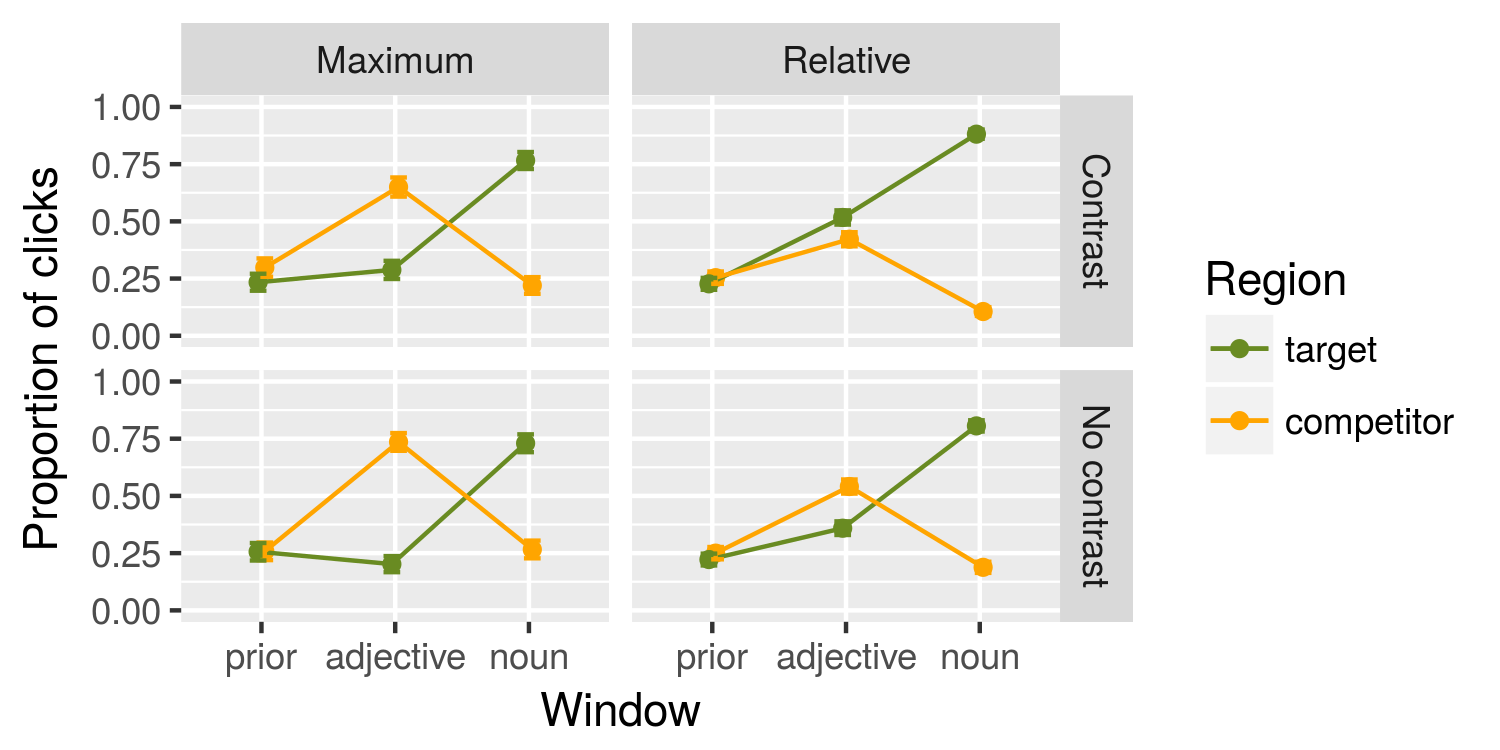
\includegraphics[width=.6\textwidth]{plots/clickdat.png}
  \caption{Proportions of clicks on the targets and competitors in the incremental decision task in different
    windows (x-axis), for different adjective types (columns) across contrast conditions (rows). Error bars indicate 95\% CIs.}
  \vspace{-4ex}
  \label{fig:clickdata}
\end{figure}

\subsection{Results}


\noindent \textbf{Clicks} \quad
Proportions of clicks on targets and competitors for different adjective types and conditions are shown in Fig.~\ref{fig:clickdata}. 
In the prior window (i.e., right after the definite article \emph{the}), participants' proportions of clicks 
 on the targets and competitors were around $.25$.
In the adjective window, for maximum adjectives the majority of the clicks were on the competitor, which 
 perfectly satisfies the adjective, and fewer clicks (around $.25$) were on the target, which only loosely
 satisfies the adjective. 
In contrast, for relative adjectives, in the no-contrast condition 
 about half of the clicks were on the competitor and fewer were on the target, 
 which exhibits a lower degree of the property denoted by the adjective than the competitor, whereas in the no-contrast condition the reverse was the case: about half of the clicks were on the target and fewer were on the competitor.
Finally, in the noun window, the vast majority of the clicks were on the target.%
\footnote{Not all of the clicks were on target, apparently because participants found that some of Leffel et al.'s stimuli did not unambiguously pick out the intended referent.
For example, some participants clicked on a perfectly straight arrow when they saw it alongside a slightly bent line with the request ``please click on the straight line''. Several participants commented that their partner seemed to be using ``line'' to descibe arrows, and similarly for certain other shapes.}
 
%\begin{figure}[ht]
%  \centering
%  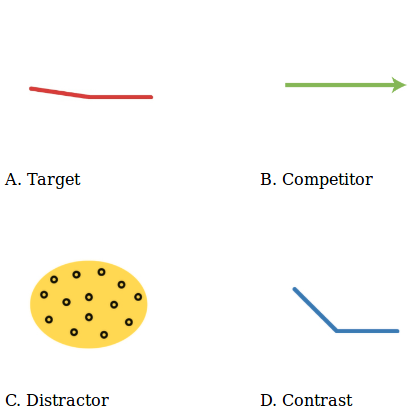
\includegraphics[width=.3\textwidth]{plots/scene18c.png}
%  \caption{A confusing trial: ``Please click on the straight line''}
%  \label{fig:confusing}
%\end{figure}


\begin{figure}[ht]
  \centering
  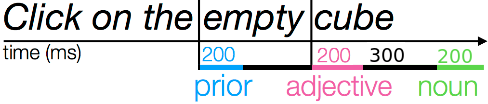
\includegraphics[width=0.3\textwidth]{plots/windows.png}
  \caption{The 3 windows used in the eye-tracking data} 
  \label{fig:windows}
\end{figure}


\noindent \textbf{Clicks vs looks} \quad
To test the linking assumption that the proportion of looks to an object reflects the probability 
 that the listener assigns to the object being the intended referent, 
 we reanalyzed the eye-tracking data from \citeNP{LeffelXiangKennedy2016:Imprecision-is-Pragmatic-}
 in 3 time windows: prior, adjective, and noun: the prior window is the first 200ms after the onset of the adjective, during which the information of the adjective has not yet been reflected in eye movement due to
 planning; the adjective window is the first 200ms after the onset of the noun; the noun window 
 is 500--700ms after the onset of the noun (Fig.~\ref{fig:windows}).
The windows were chosen so that the click data and the eye-tracking data are maximally comparable: they
 were late enough so that the previous information had been processed as much as possible
 yet without the influence of the new information, making it close to the offline task that has no time limit. 



\begin{figure}[ht]
  \centering
  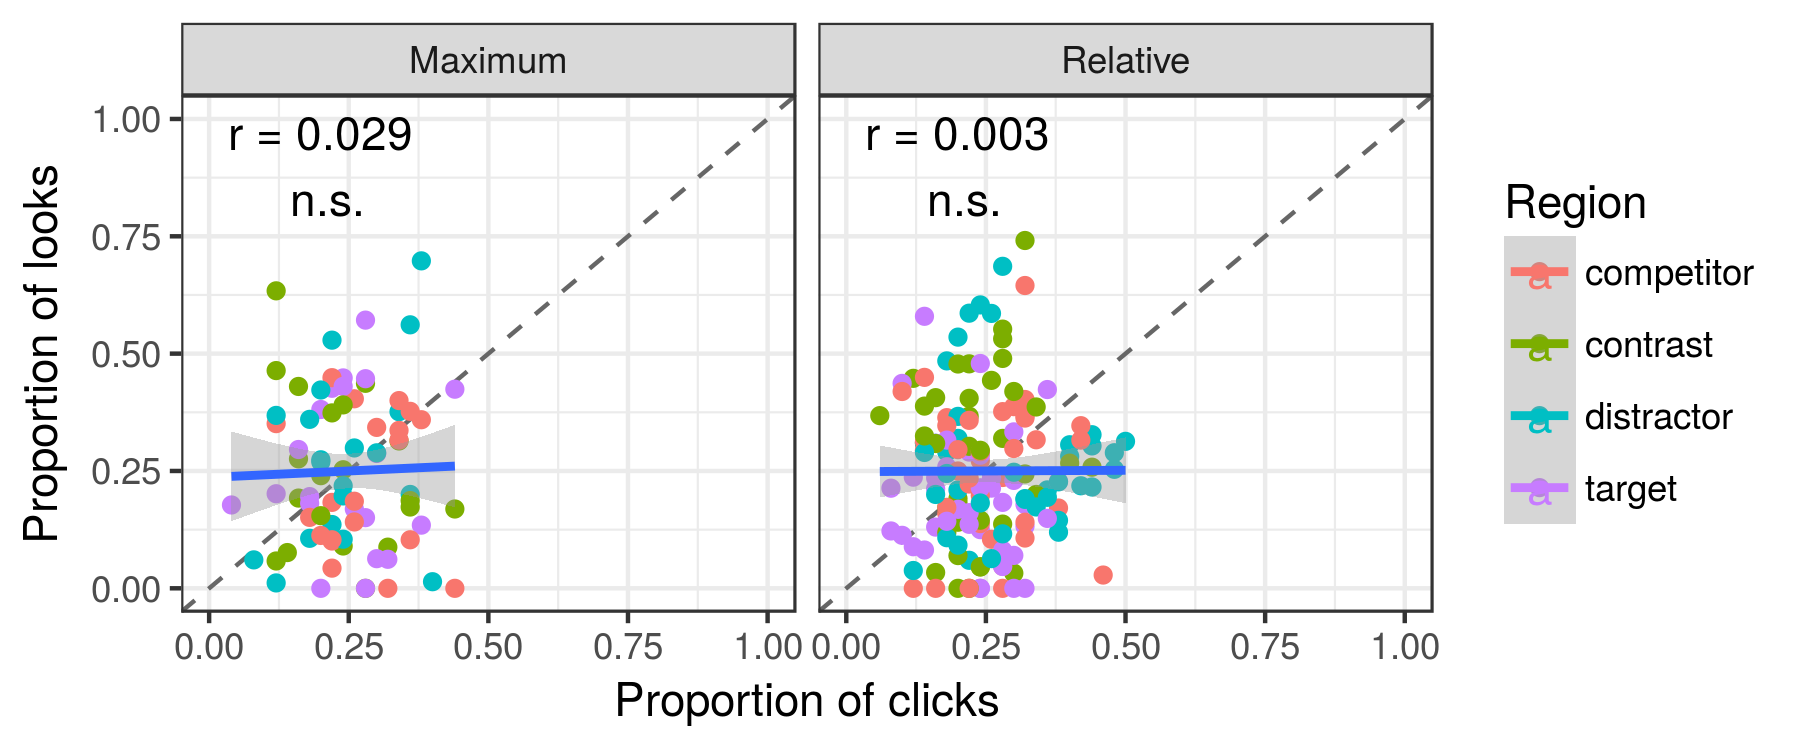
\includegraphics[width=0.5\textwidth]{plots/prior.png}
  \caption{Correlations between click and eye movement data in the prior window
    for different adjective types (columns)} 
  \label{fig:priorcors}
\end{figure}

In the prior window (Fig.~\ref{fig:priorcors}), we observed no significant correlations between proportion of looks 
and proportion of clicks on an object ($r<.03, p > .1$ for both adjective types).


\begin{figure}[ht]
  \centering
 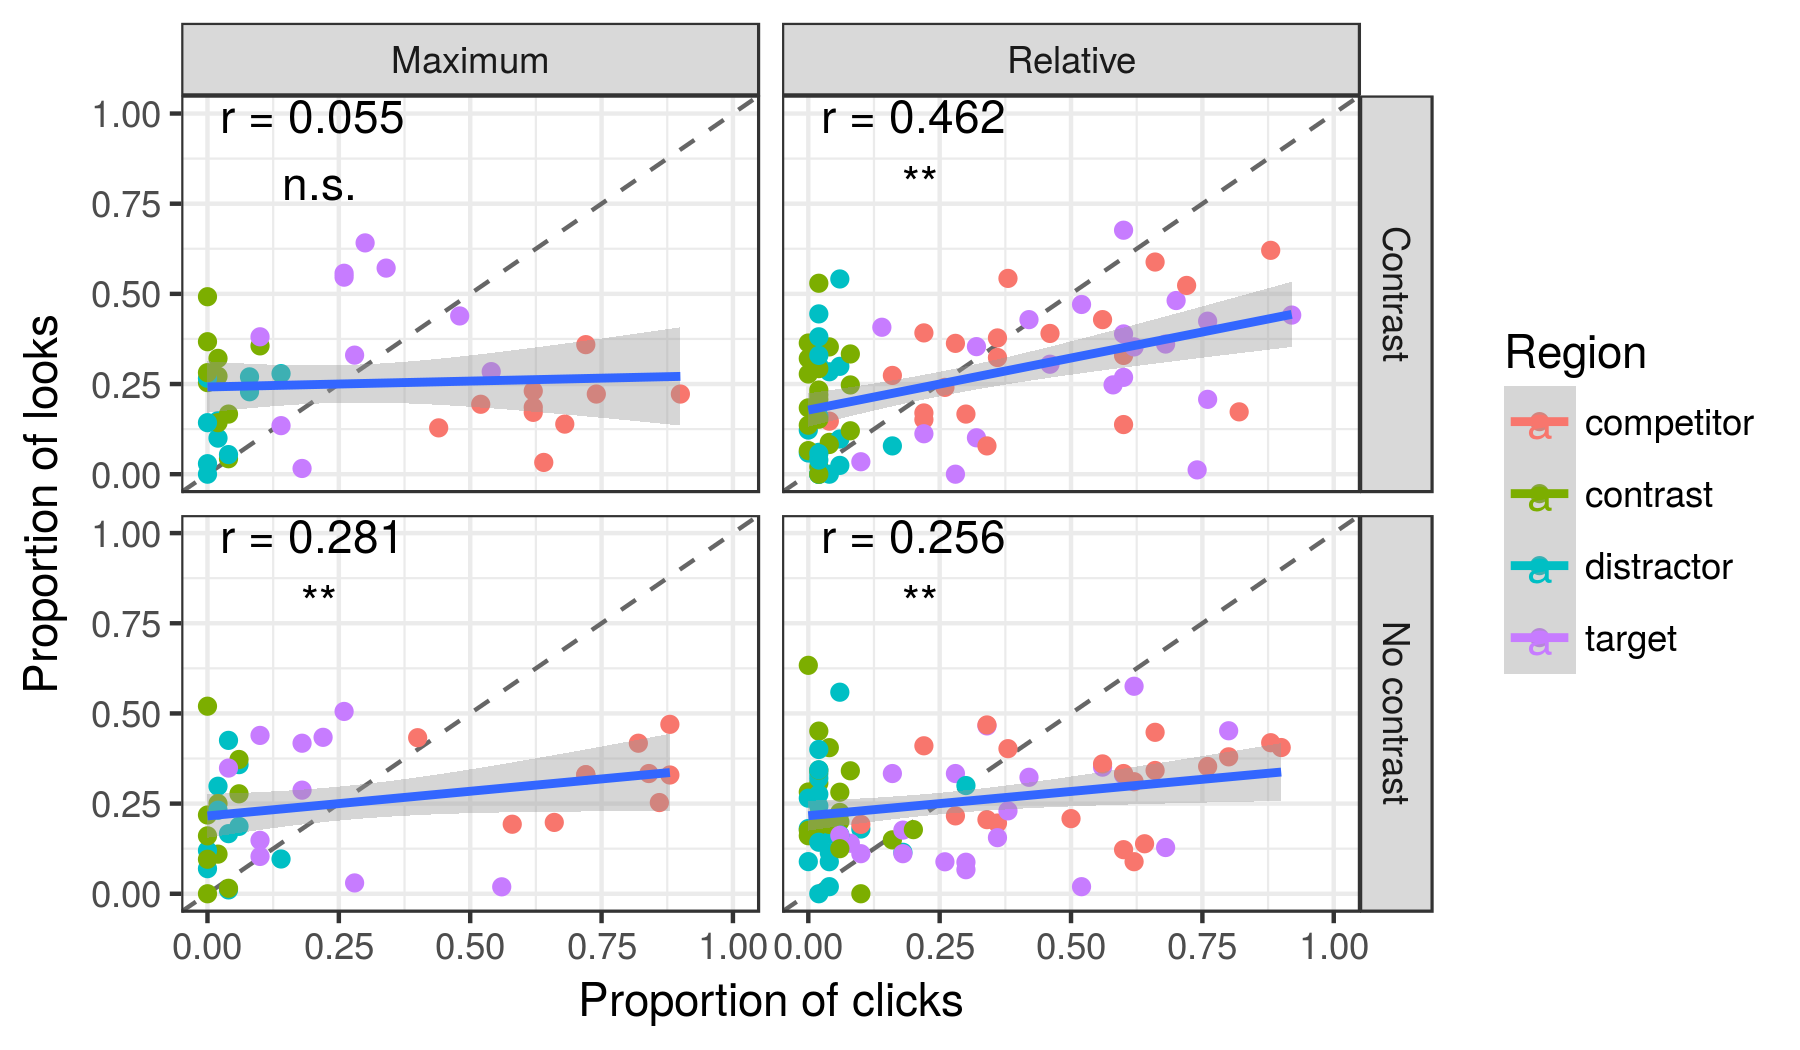
\includegraphics[width=.5\textwidth]{plots/adjBrokenDown.png}
 \caption{Correlations between click and eye movement data in the adjective window for 
   different adjective types (columns) and contrast conditions (rows)}
 \label{fig:adjcors}
\end{figure}



In the adjective window (Fig.~\ref{fig:adjcors}), in the contrast condition, 
 we observed no significant correlation between proportions of clicks and looks for maximum adjectives ($r = .055, p >.1$) but a medium correlation for relative adjectives ($r = .462, p < .01$).
In the no-contrast condition, we observed a weak correlation for both maximum ($r = .281, p < .01$) 
 and relative ($r = .256, p < .01$) adjectives. 


\begin{figure}[ht]
  \centering
  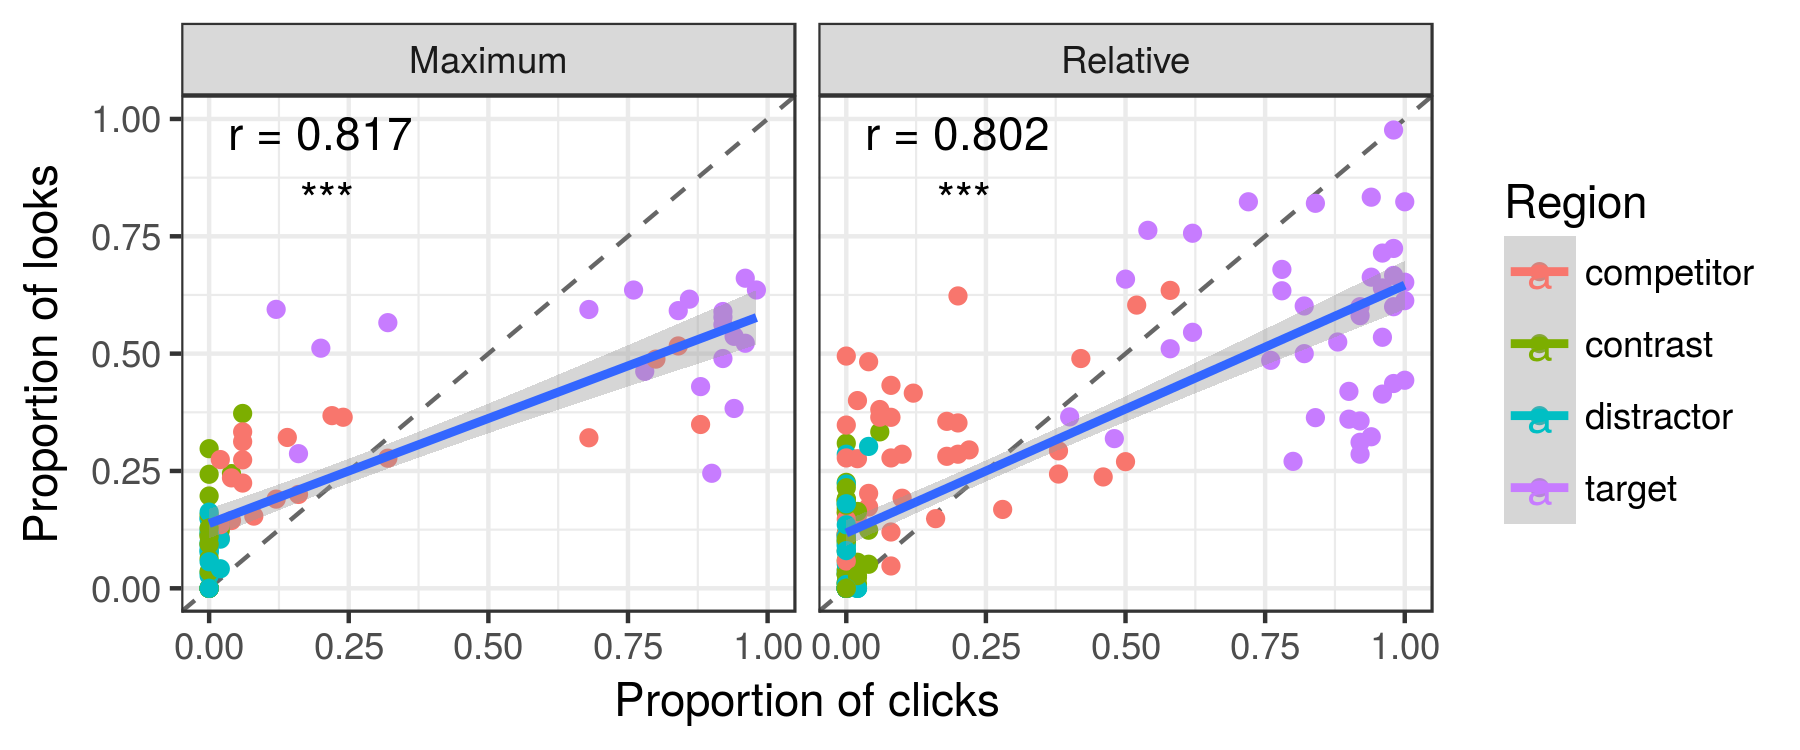
\includegraphics[width=0.5\textwidth]{plots/noun.png}
  \caption{Correlations between click and eye movement data in the noun window
    for different adjective types (columns)} 
  \vspace{-2ex}
  \label{fig:nouncors}
\end{figure}

In the noun window (Fig.~\ref{fig:nouncors}), we observed a strong correlation 
 between proportions of clicks and looks for both maximum 
 and relative adjectives ($r > .8, p < .001$). 

% free production stimuli and plots
\begin{figure*}[ht]
  \centering
  \begin{subfigure}[b]{0.55\textwidth}
    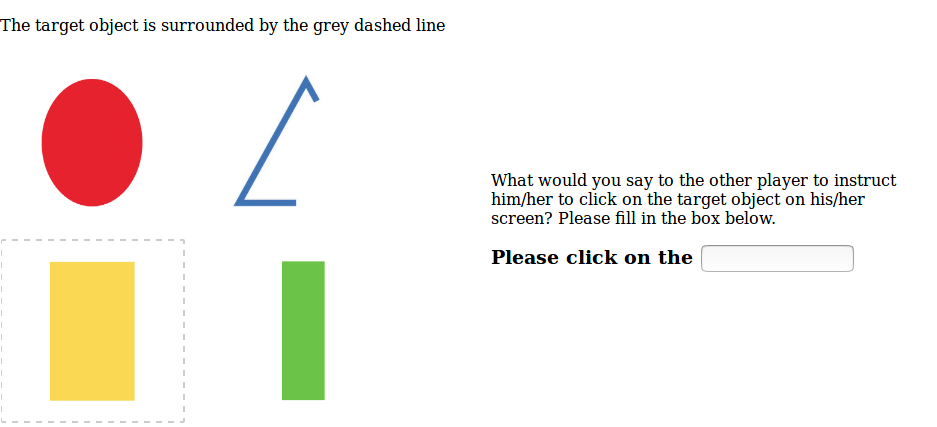
\includegraphics[width=\textwidth]{plots/freeprodTurk.png}
    \caption{Sample stimuli}
    \label{fig:freeprodturk}
  \end{subfigure}
  ~ %add desired spacing between images, e. g. ~, \quad, \qquad, \hfill etc. 
  %(or a blank line to force the subfigure onto a new line)
  \begin{subfigure}[b]{0.4\textwidth}
    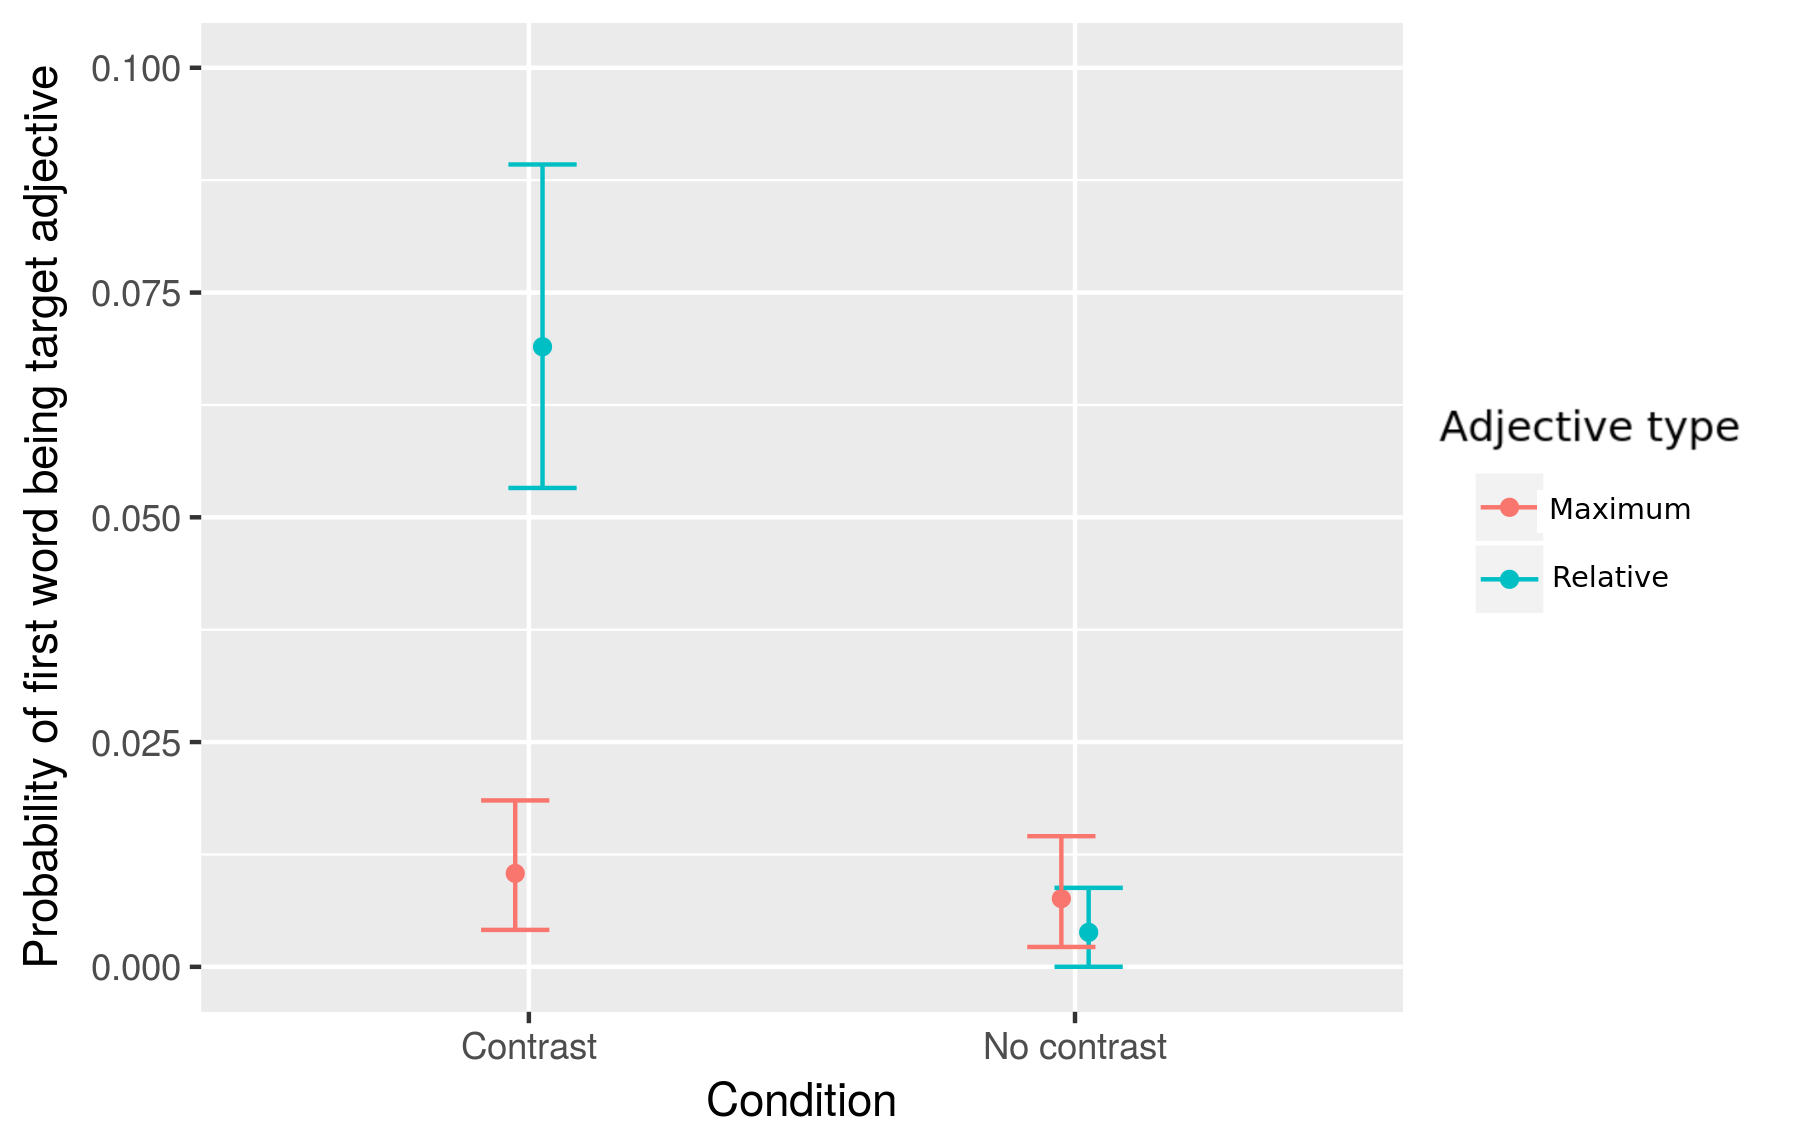
\includegraphics[width=\textwidth]{plots/freeprodPlot.png}
    \caption{Proportions of first word being the target adjective}
    \label{fig:freeprodplot}
  \end{subfigure}
  %  ~ %add desired spacing between images, e. g. ~, \quad, \qquad, \hfill etc. 
  %  %(or a blank line to force the subfigure onto a new line)
  %  \begin{subfigure}[b]{0.2\textwidth}
  %    \includegraphics[width=\textwidth]{mouse}
  %    \caption{A mouse}
  %    \label{fig:mouse}
  %  \end{subfigure}
  \caption{The free production experiment and results (error bars indicate 95\% CIs)}
  \vspace{-2ex}
  \label{fig:freeprod}
\end{figure*}

\subsection{Discussion}

The results suggest that the degree to which an object is believed to be the referent correlates with the 
 proportion of looks on that object to various extents depending both on the window and the adjective type. 
 
As the sentence unfolds, the correlation between clicks and looks generally increases.
This is likely due to a tradeoff between \emph{exploration} and \emph{exploitation}: In earlier windows, participants were less
 familiar with the objects. Thus, they were likely mainly exploring the scene, resulting in eye movements that were not signal-driven, and consequently their proportions of looks did not necessarily correlate with their belief about the intended referent.
In contrast, in later windows participants were more familiar with the objects and might have had more resources available for exploiting their signal-driven beliefs.

We also observed that in the adjective window, adjective type affects 
 the correlation between clicks and looks and the correlations are relatively low compared with \citeauthor{AllopennaEtAl1998:Tracking-the-Time-}'s results.
Note that in \citeauthor{AllopennaEtAl1998:Tracking-the-Time-}'s studies, participants were trained to name all the items so they had no uncertainty 
 about how the target would be called, whereas the adjectives in \citeauthor{LeffelXiangKennedy2016:Imprecision-is-Pragmatic-}'s experiments
 were probably less expected because modification was not necessary in the no-contrast conditions and presumably color adjectives were more likely modifiers.
Therefore we hypothesized that the differences in correlations were due to  different expectations of hearing the adjectives.
If participants hear a less expected adjective, they will need to explore the scene more, e.g., to evaluate
whether each object satisfies the adjective, and hence the correlation between proportions of looks and 
beliefs will be lower.
If participants hear a more expected adjective, they can directly exploit the signal, and hence 
 the correlation between proportions of looks and beliefs will be higher.
Given that it is easy to shift the standard $\theta$ in light of the local comparison between the target and the contrast objects for relative adjectives but difficult to do so for maximum adjectives  
 \cite{SyrettKennedyLidz2010:Meaning-and-Context-}, and given that there is no need to use an adjective in the no-contrast condition, we
hypothesized that adjectives were most expected in the contrast condition for relative adjectives.

To test this hypothesis, we conducted a free production experiment on Amazon Mechanical Turk to measure the 
 likelihood of the participants describing the target using the adjective in \citeauthor{LeffelXiangKennedy2016:Imprecision-is-Pragmatic-}'s original experiment and Exp~1.





\section{Experiment 2: Free production task}



\subsection{Methods}

Using the same stimuli as in Exp.~1, 100 self-identified native English speakers were told that they were playing a game with a partner
 and 
 their task was to instruct their partner to click on the target object, which was surrounded by the 
 grey dashed line that their partner could not see. 
To familiarize the participants with the task, they first played 8 listener trials similar to Exp~1 
 but only with full sentences,
 then practiced 1 speaker trial, and finally played 30 speaker trials where they completed the sentence 
 ``please click on the \underline{\quad}'' for either the target or the competitor in the critical trials in
 Exp~1. 
They were told not to mention colors or locations to make the game more challenging. (In a pilot study without this restriction, almost all the adjectives in the responses were color terms.) 


\subsection{Results} 

Fig.~\ref{fig:freeprodplot} shows the proportions of descriptions of the target object 
 in which the first word was the adjective used 
 in \citeauthor{LeffelXiangKennedy2016:Imprecision-is-Pragmatic-}'s original experiment and Exp~1 
 (referred to as the target adjective).
The target adjective was used the most in the contrast condition for relative adjectives, and in the 
other three cases the target adjective was used less.
Note that the target adjective was not likely to be used right after the definite article
 (probabilities $<$.1 in all four cases). 
Instead, participants often used comparative forms (e.g., \emph{wider rectangle}), 
 modifiers (e.g., \emph{almost empty cube}), and sometimes different adjectives (e.g., \emph{big} instead of \emph{tall}/\emph{wide}). 

\subsection{Discussion}

The results provide some initial support for our hypothesis that expectations of the adjectives also play 
 a role in the correlation between looks and clicks.
The target adjective was more likely to be used right after the definite article \emph{the}
 in the contrast condition for relative adjectives than in the other 3 cases, therefore
 it was most expected by the listener and indeed the correlation between looks and clicks was the highest for relative adjectives in the contrast condition.
However, note that in the other 3 cases since the target adjective was very unlikely to be mentioned 
 (probabilities $< .02$), we do not have enough evidence to determine whether expectations of adjectives can 
 account for their different correlations.
 

 
\section{General discussion}

Our results suggest that at least in this dataset, the linking hypothesis stated previously is only partially supported:
 the degree to which an object is believed to be the referent is only one factor that affects eye movements in referential tasks in which participants' goal is to interact with the intended referent; 
 utterance expectations also play a role in this referential task. 
This has methodological implications for how proportions of looks in visual-world eye-tracking
 experiments should be interpreted. 
 
Experimental results that manipulation X induces more looks on the target are often characterized as the manipulation facilitating reference resolution, which in turn often
 implies that manipulation X induces a stronger belief that the target is the intended referent \cite<e.g.,>[among many others]{LeffelXiangKennedy2016:Imprecision-is-Pragmatic-,Mulders2016,Kurumada2015,SalverdaTanenhaus2017:The-Visual-World-Paradigm}.
However, this interpretation is valid only if the correlation between beliefs and looks is constant 
 across manipulation X. Our results show that this may not always be the case.
Therefore, additional caution is needed to make sure that empirical measures such as proportions of looks 
 actually track the theoretical constructs that researchers are interested in.
For example, without testing the linking hypothesis, one might look at \citeauthor{LeffelXiangKennedy2016:Imprecision-is-Pragmatic-}'s results in Fig~\ref{fig:leffelEtAlResults}
 and conclude from more looks on the target in the adjective window in the contrast condition for maximum adjectives that participants preferred the imprecise interpretation of maximum adjectives in the presence of
 contrast.\footnote{Note that \citeA{LeffelXiangKennedy2016:Imprecision-is-Pragmatic-} did not make this claim.} 
This is at odds with the results from our offline incremental decision task that directly measured participants'
 beliefs (Fig.~\ref{fig:clickdata}).

We note that our study is only a first stab at testing explicit linking hypotheses used in visual-world
 eye-tracking studies.
Further research is required to assess to what extent these results are robust and generalizable across eye movement datasets in experimental linguistics, 
but we believe that the offline incremental decision task provides a promising way to start investigating such 
problems.
We are focusing on referential tasks where participants are instructed to interact with the referent.
Such tasks can be straightforwardly adapted to offline incremental decision tasks and the correlations between
 clicks and looks can be tested.
It would also be interesting to extend and apply the offline incremental decision task to
 passive-listening  tasks to test correlations between looks and listeners' beliefs about the current 
 or upcoming referent.
Finally, the offline incremental decision task might be useful to test other linking hypotheses.


%\vspace{-1ex}

\section{Conclusion}

In this paper, we supplemented the eye-tracking data from \citeA{LeffelXiangKennedy2016:Imprecision-is-Pragmatic-} with an offline \emph{incremental decision task} to
measure participants’ beliefs about the intended referent at various points in the unfolding sentence, 
and tested a simple, explicit linking hypothesis: the proportion of looks to an object correlates with the probability that the listener assigns to the object being the target.
Our results suggest that the degree to which an object is believed to be the referent is only one factor that affects eye movements in referential tasks. Preliminary free production data we have collected for the scenes suggests that utterance expectations also play a role in determining the correlation between clicks and looks.
When the adjective is most expected, we observed the highest correlations, i.e., 
beliefs were a better predictor of eye-movements. 
Based on these results, we argue that proportions of looks in visual-world eye-tracking experiments should be 
 interpreted with more caution and suggest stating the linking hypothesis explicitly and test it 
 using the incremental decision task.



\section{Acknowledgments}

We are very grateful to Tim Leffel, Ming Xiang, and Chris Kennedy for generously sharing their data and stimuli.

%\section{Formalities, Footnotes, and Floats}
%
%Use standard APA citation format. Citations within the text should
%include the author's last name and year. If the authors' names are
%included in the sentence, place only the year in parentheses, as in
%\citeA{NewellSimon1972a}, but otherwise place the entire reference in
%parentheses with the authors and year separated by a comma
%\cite{NewellSimon1972a}. List multiple references alphabetically and
%separate them by semicolons
%\cite{ChalnickBillman1988a,NewellSimon1972a}. Use the
%``et~al.'' construction only after listing all the authors to a
%publication in an earlier reference and for citations with four or
%more authors.
%
%
%\subsection{Footnotes}
%
%Indicate footnotes with a number\footnote{Sample of the first
%  footnote.} in the text. Place the footnotes in 9~point type at the
%bottom of the column on which they appear. Precede the footnote block
%with a horizontal rule.\footnote{Sample of the second footnote.}


%\subsection{Tables}
%
%Number tables consecutively. Place the table number and title (in
%10~point) above the table with one line space above the caption and
%one line space below it, as in Table~\ref{sample-table}. You may float
%tables to the top or bottom of a column, or set wide tables across
%both columns.
%
%\begin{table}[!ht]
%  \begin{center} 
%    \caption{Sample table title.} 
%    \label{sample-table} 
%    \vskip 0.12in
%    \begin{tabular}{ll} 
%      \hline
%      Error type    &  Example \\
%      \hline
%      Take smaller        &   63 - 44 = 21 \\
%      Always borrow~~~~   &   96 - 42 = 34 \\
%      0 - N = N           &   70 - 47 = 37 \\
%      0 - N = 0           &   70 - 47 = 30 \\
%      \hline
%    \end{tabular} 
%  \end{center} 
%\end{table}


%\subsection{Figures}
%
%All artwork must be very dark for purposes of reproduction and should
%not be hand drawn. Number figures sequentially, placing the figure
%number and caption, in 10~point, after the figure with one line space
%above the caption and one line space below it, as in
%Figure~\ref{sample-figure}. If necessary, leave extra white space at
%the bottom of the page to avoid splitting the figure and figure
%caption. You may float figures to the top or bottom of a column, or
%set wide figures across both columns.
%
%\begin{figure}[ht]
%  \begin{center}
%    \fbox{CoGNiTiVe ScIeNcE}
%  \end{center}
%  \caption{This is a figure.} 
%  \label{sample-figure}
%\end{figure}



%\section{References Instructions}
%
%Follow the APA Publication Manual for citation format, both within the
%text and in the reference list, with the following exceptions: (a) do
%not cite the page numbers of any book, including chapters in edited
%volumes; (b) use the same format for unpublished references as for
%published ones. Alphabetize references by the surnames of the authors,
%with single author entries preceding multiple author entries. Order
%references by the same authors by the year of publication, with the
%earliest first.
%
%Use a first level section heading, ``{\bf References}'', as shown
%below. Use a hanging indent style, with the first line of the
%reference flush against the left margin and subsequent lines indented
%by 1/8~inch. Below are example references for a conference paper, book
%chapter, journal article, dissertation, book, technical report, and
%edited volume, respectively.

%\nocite{ChalnickBillman1988a}
%\nocite{Feigenbaum1963a}
%\nocite{Hill1983a}
%\nocite{OhlssonLangley1985a}
%% \nocite{Lewis1978a}
%\nocite{Matlock2001}
%\nocite{NewellSimon1972a}
%\nocite{ShragerLangley1990a}


\bibliographystyle{apacite}

\setlength{\bibleftmargin}{.125in}
\setlength{\bibindent}{-\bibleftmargin}

\bibliography{GAVisualWorld}


\end{document}
